\documentclass[10pt,twocolumn]{article}

\usepackage[letterpaper,top=0.72in,bottom=0.78in,left=0.70in,right=0.70in]{geometry}
\usepackage[T1]{fontenc}
\usepackage{lmodern}
\usepackage{microtype}
\usepackage{graphicx}
\usepackage{booktabs}
\usepackage{amsmath,amssymb}
\usepackage{xcolor}
\usepackage{authblk}
\usepackage{caption}
\usepackage{enumitem}
\usepackage{fancyhdr}
\usepackage{natbib}
\usepackage{balance}
\usepackage[hidelinks]{hyperref}

\definecolor{ink}{HTML}{173042}
\definecolor{teal}{HTML}{2A9D8F}
\definecolor{coral}{HTML}{E76F51}
\definecolor{muted}{HTML}{687780}

\hypersetup{
  colorlinks=true,
  linkcolor=ink,
  citecolor=teal,
  urlcolor=coral,
  pdftitle={Single-neuron response strength and latency predict held-out group currents},
  pdfauthor={Javier Emilio Bazan Sanchez}
}

\graphicspath{{figures/}}
\setlength{\columnsep}{0.24in}
\setlength{\parindent}{1em}
\setlength{\parskip}{0pt}
\setlist{nosep,leftmargin=*}
\captionsetup{font=small,labelfont=bf}
\pagestyle{fancy}
\fancyhf{}
\fancyhead[L]{\footnotesize Bazan Sanchez}
\fancyhead[R]{\footnotesize Single-neuron response model}
\fancyfoot[C]{\thepage}
\renewcommand{\headrulewidth}{0.3pt}

\title{\color{ink}\bfseries Single-neuron response strength and latency predict held-out group currents}
\author[1]{Javier Emilio Bazan Sanchez\thanks{Correspondence: \href{mailto:bazan@ciencias.unam.mx}{bazan@ciencias.unam.mx}}}
\affil[1]{Faculty of Sciences, National Autonomous University of Mexico (UNAM), Mexico City, Mexico}
\date{Preprint \textbar{} \today}

\begin{document}

\raggedbottom

\maketitle

\begin{abstract}
Public cortical-slice recordings pair two-photon stimulation of individual
neurons with stimulation of groups of neurons while postsynaptic current is
recorded from one patched cell. These data were used to test whether
single-neuron responses predict held-out group responses. For each laser
power, a response shared across neurons was estimated first. Repeatable
neuron-specific differences were then learned from two halves of the
single-neuron trials and added to predict group trials; no group response was
used for fitting.

The rule was developed in nine somatostatin-to-excitatory (SST-to-E) files
and frozen before the excitatory-to-excitatory (E-to-E) files were opened.
The E-to-E cohort contained 129,613 single-neuron trials and 74,435
group trials across ten recorded cells. The reliability-weighted model
improved demixed-current mean-squared error (MSE) over a power-only baseline
in all ten files (mean gain $2.12\times10^{-5}$, $q=0.00195$). Correct neuron
identity was necessary in shuffle and replacement controls. A post-feedback
comparison showed that source-specific response strength explained 96.7\% of
the MSE improvement; adding a source-specific latency shift explained nearly
all of it. The full waveform improved correlation over power alone, but not
conclusively over strength plus latency. In raw current, the full waveform did
not improve correlation, but the simpler gain-plus-latency model did so in all
ten files in the post-feedback analysis. The public files do not identify
animal or slice membership, so inferential tests are reported at the file
level and a three-date clustering is included as a conservative sensitivity
analysis.
\end{abstract}

\noindent\textbf{Keywords:} two-photon holographic optogenetics;
postsynaptic current; single-neuron stimulation; held-out prediction;
source-specific response strength; response latency; neural waveform demixing

\begin{table*}[t]
  \centering
  \caption{\textbf{Terminology.} Definitions used throughout the paper.}
  \label{tab:glossary}
  \begin{tabular}{@{}p{0.19\textwidth}p{0.76\textwidth}@{}}
    \toprule
    Term & Meaning in this study \\
    \midrule
    Single-neuron trial & A trial in which exactly one neuron is stimulated;
    these trials are used to learn responses. \\
    Group trial & A trial in which several neurons are stimulated together;
    these trials are held out to test predictions. \\
    Shared response & The part of the waveform that is common across neurons
    stimulated at the same laser power. \\
    Neuron-specific\newline difference & The part that distinguishes one stimulated
    neuron from the shared response. \\
    Reliability $\lambda_p$ & The fraction of neuron-specific detail kept
    because it repeats across two halves of the single-neuron trials. \\
    Recording file & One patched postsynaptic cell, its candidate stimulated
    neurons, the stimulation design, and the recorded current trials. \\
    Demixed current & Current after neural waveform demixing (NWD), a
    source-identity-blind U-Net that suppresses overlapping events and noise. \\
    Power-only baseline & A prediction that knows the laser power of each
    stimulus but not which neurons were stimulated. \\
    \bottomrule
  \end{tabular}
\end{table*}

\section{Introduction}

Observing neural activity does not by itself show what a neuron contributes
when it is activated. Two-photon holographic optogenetics provides a direct
test: selected neurons can be stimulated individually or together while the
current entering a patched postsynaptic neuron is recorded
\citep{packer2012two,packer2015simultaneous,mardinly2018precise,
adesnik2021probing}.

The public data analyzed here come from cortical slices \citep{gajowa2025dataset,
triplett2025rapid}. Each file represents one patched postsynaptic cell and
contains hundreds of candidate neurons distributed across four or five
imaging depths. On each trial, a matrix records which candidates were
stimulated and at what laser power. The file also contains the resulting
45-ms current trace in raw form and after neural waveform demixing (NWD).
Trials stimulating one candidate can therefore be used for learning, while
trials stimulating groups can be reserved for evaluation.

The source study used CAVIaR to predict a held-out hologram after fitting
responses to other group holograms \citep{triplett2025rapid}. The contrast
here is narrower: no group response is used for fitting. The question is
whether responses learned only from single-neuron trials transfer when those
neurons are stimulated in groups.

Let $s$ identify the stimulated neuron, $p$ the laser power, and $t$ the time
after stimulation. Repeated trials showed that some apparent differences
between neurons were unstable. The model keeps only the repeatable part of
the single-neuron response:
\begin{align}
r_{s,p}(t) &= g_p(t) + \lambda_p d_{s,p}(t), \label{eq:response}\\
\widehat{y}_{E}(t) &= \sum_{s\in E} r_{s,p_s}(t), \label{eq:sum}
\end{align}
Here, $g_p(t)$ is the response shared across neurons at power $p$,
$d_{s,p}(t)$ is the difference for neuron $s$, and $\lambda_p$ measures how
well those differences repeat across two halves of the single-neuron trials
(Fig.~\ref{fig:model}). Unreliable differences are reduced and reliable
differences are retained. The model then adds the learned responses of all
stimulated neurons. Group responses are used only for testing, never for
fitting.

The order of the analysis matters. A planned first model improved MSE but
missed its waveform-correlation criterion in SST-to-E recordings. The
already-open SST data were then used to develop the reliability rule. The new
rule was frozen before the E-to-E dataset was downloaded or inspected.
The first dataset was used for development; the second provided a
prospectively held-out test at the recording-file level.

\begin{figure*}[t]
  \centering
  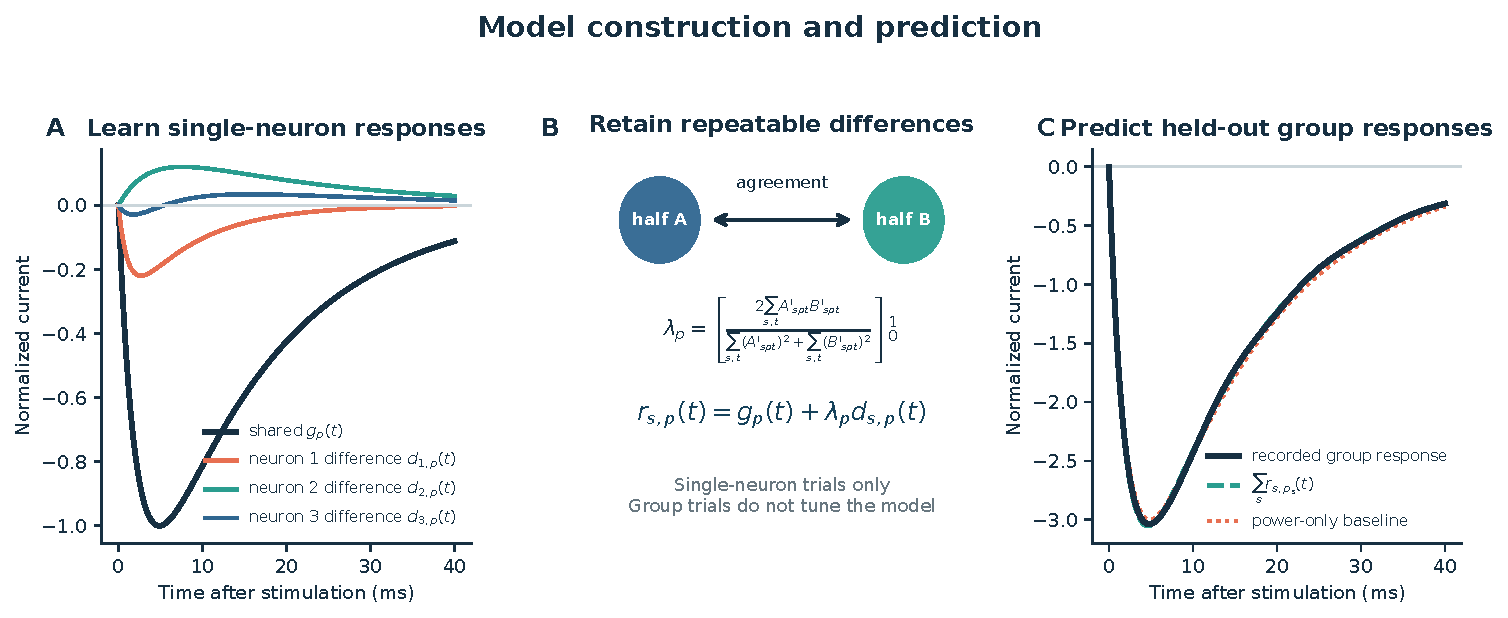
\includegraphics[width=\textwidth]{figure1_grammar.pdf}
  \caption{\textbf{The prediction rule.}
  \textbf{A}, At each laser power, the mean response to one neuron is split
  into a shared waveform $g_p(t)$ and a neuron-specific difference
  $d_{s,p}(t)$. Curves are schematic. \textbf{B}, Two alternating halves of
  the trials estimate reliability $\lambda_p$. Repeatable differences are
  kept; unstable differences are reduced. \textbf{C}, The model adds the
  learned responses of the stimulated neurons and tests the prediction on group
  trials that were not used for fitting.}
  \label{fig:model}
\end{figure*}

\section{Results}

\subsection{The recordings pair learning trials with held-out group trials}

The nine SST-to-E files record stimulation of somatostatin neurons while
current is measured from an excitatory postsynaptic cell. The ten E-to-E
files record stimulation of excitatory neurons while current is measured from
another excitatory cell. Each file contains one recorded postsynaptic cell,
214--687 candidate stimulated neurons, four or five imaging depths, a
trial-by-neuron stimulation matrix, and raw and NWD-demixed current. Across
the E-to-E cohort there were 4,724 candidate-neuron entries and 204,054
trials. Exactly one neuron was stimulated in 129,613 trials; more than one
was stimulated in 74,435 trials; six blank trials were excluded.

The distinction between trial types defines the prediction task.
Single-neuron trials estimate each neuron's response. Group trials test the
sum of those estimates. A group trial is eligible only when every stimulated
neuron has at least three single-neuron trials at the exact delivered power.
All 74,435 E-to-E group trials met this rule (Table~\ref{tab:dataset}).

\begin{table*}[t]
  \centering
  \caption{\textbf{Dataset overview.} Technical characteristics of the
  prospectively held-out E-to-E recordings used for the main file-level test.}
  \label{tab:dataset}
  \begin{tabular}{@{}p{0.20\textwidth}p{0.35\textwidth}p{0.39\textwidth}@{}}
    \toprule
    Component & Recorded data & Role in the analysis \\
    \midrule
    Preparation & Acute cortical slices; excitatory candidate neurons were
    stimulated while current was recorded from one patched excitatory neuron
    per file. & Tests excitatory-to-excitatory transfer of responses measured
    under controlled stimulation. \\
    Recording units & 10 files, each representing one labeled postsynaptic
    cell; 4,724 candidate-neuron entries, with 214--687 candidates per file. &
    File means are the inferential units because animal and slice identifiers
    are unavailable. \\
    Spatial sampling & Candidates distributed across four or five two-photon
    imaging depths in each file; coordinates are stored in
    \texttt{targets}. & Depth is retained in identity-matched controls and
    null permutations. \\
    Stimulation design & \texttt{stimulus\_matrix} has one row per trial and
    one column per candidate neuron; positive entries give the delivered laser
    power. & Defines the stimulated set, group size, neuron identity, and exact
    source--power pairs. \\
    Current traces & 900 samples per trial at 20 kHz (45 ms), stored as raw
    current in \texttt{pscs} and NWD-demixed current in
    \texttt{pscs\_demixed}. & Demixed current is the primary outcome; raw
    current provides a preprocessing sensitivity analysis. \\
    Single-neuron trials & 129,613 trials with exactly one positive stimulus
    entry. & Estimate shared and neuron-specific responses, reliability,
    source gain, and source latency. \\
    Group trials & 74,435 trials with more than one positive stimulus entry;
    all satisfy the minimum-data eligibility rule. & Held out from fitting and
    used only to evaluate predictions. \\
    Blank trials & 6 trials with no stimulated candidate and nonfinite current
    traces. & Excluded before response estimation or evaluation. \\
    Biological metadata & 10 recorded-cell labels across three acquisition
    dates; slice and animal membership are not provided. & Main tests are
    file-level; acquisition date is used only as a conservative clustering
    sensitivity. \\
    \bottomrule
  \end{tabular}
\end{table*}

\subsection{The first test revealed unstable waveform detail}

The first test used nine checksum-verified SST-to-E files with 46,578 trials.
Of these, 26,803 stimulated one neuron and 19,769 stimulated groups. A total
of 19,217 group trials had enough single-neuron data to make a prediction.
The first model added the full mean waveform for each stimulated
neuron. The baseline ignored neuron identity and added the shared mean
response at each delivered power.

Using neuron identity improved demixed response-window MSE over the baseline
in all nine files (mean file gain $8.78\times10^{-4}$, exact
$p=0.001953$, Benjamini--Hochberg $q=0.003906$). However, it did not improve
waveform correlation (mean $\Delta\rho=-0.00263$, $p=0.682$,
$q=0.682$). The plan required both measures to improve, so fourteen PV-to-E
files remained unopened (Fig.~\ref{fig:path}). Neuron identity still carried
information about response size. The failed waveform criterion motivated
separating repeatable neuron-specific detail from trial-to-trial noise.

\begin{figure*}[t]
  \centering
  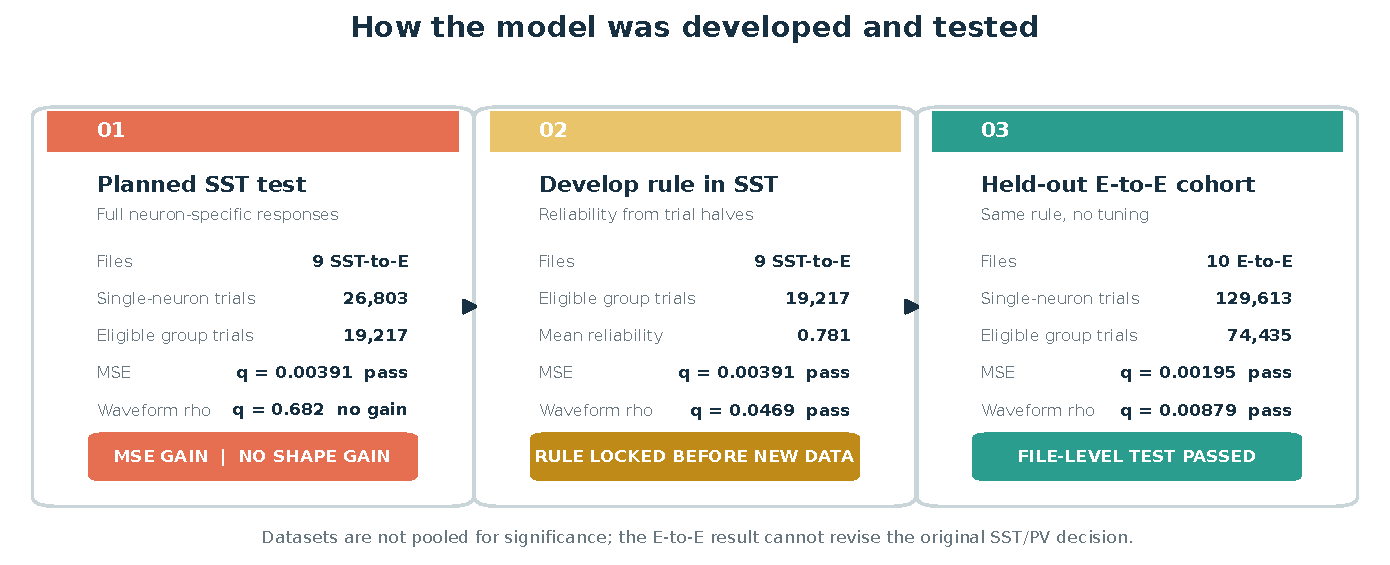
\includegraphics[width=\textwidth]{figure2_evidence_path.pdf}
  \caption{\textbf{Order of the analysis.} The first SST test improved MSE
  but not waveform correlation, so PV data remained unopened. The
  reliability rule was developed only in the already-open SST data. The rule
  and its success criteria were frozen before the E-to-E data were opened.
  Results are not pooled across stages or datasets.}
  \label{fig:path}
\end{figure*}

\subsection{Repeatability identified which details to keep}

An exploratory follow-up tested whether repeatability identified
neuron-specific responses that improved group-response prediction. Median
split-half reliability closely tracked the gain in waveform correlation
across the nine files (Spearman $\rho=0.957$). This observation was exploratory
because the SST group responses had already been opened. For the new rule,
alternating trials provided two independent estimates of the neuron-specific
differences. Their agreement determined $\lambda_p$, from 0 for no retained
detail to 1 for the full difference (Methods).

The model kept 78.1\% of the neuron-specific difference on average in the
demixed SST responses ($\lambda=0.781$). It improved both MSE (mean
$8.92\times10^{-4}$, $q=0.003906$) and waveform correlation (mean $0.00413$,
$q=0.04688$) over the baseline. Both improvements remained positive when
each file was removed in turn. Identity-shuffling controls passed, and
replacing a stimulated neuron with a matched unstimulated neuron increased
MSE in all nine files. These results helped develop the model, but they were
not a held-out confirmation. They established the
reliability-weighted rule to be tested in new data, while the PV files
remained unopened under the original protocol.

\begin{table*}[t]
  \centering
  \caption{\textbf{The three stages of the analysis.} Effects are file-level
  means for the neuron-specific model relative to the baseline that knows
  laser power but not neuron identity. The reliability-weighted SST result
  was used for development, not held-out confirmation.}
  \label{tab:cohorts}
  \resizebox{\textwidth}{!}{\begin{tabular}{@{}lllrrrr@{}}
\toprule
Model & Data & Role & MSE improvement & MSE $q$ & Correlation improvement & Correlation $q$ \\
\midrule
Full response & SST & planned first test & 8.777e-04 & 0.003906 & -0.00263 & 0.6816 \\
Reliability-weighted & SST & reliability development & 8.922e-04 & 0.003906 & 0.00413 & 0.04688 \\
Reliability-weighted & E-to-E & held-out cohort & 2.120e-05 & 0.001953 & 0.00397 & 0.008789 \\
\bottomrule
\end{tabular}
}
\end{table*}

\subsection{The frozen rule generalized to a held-out E-to-E cohort}

The prospective file-level test used all ten files in a checksum-verified E-to-E
dataset. Before the data were opened, the protocol, file manifest, and SST
development summary were locked with SHA-256 hashes. One file used the
previously unused field name \texttt{caviar\_weights\_ensemble} instead of
\texttt{caviar\_weights\_multi}. This naming difference was recorded before
response values were read; it did not change the model.

The dataset contained 204,054 trials. The 129,613 single-neuron trials were
used to learn the responses and reliability values. The 74,435 group trials
were used only to test predictions, and every group trial was eligible. The
reliability-weighted model improved demixed MSE over the baseline in all ten
files (mean gain
$2.1195\times10^{-5}$, exact $p=0.0009766$, $q=0.001953$) and waveform
correlation in 9/10 files (mean gain $0.003973$, $p=q=0.008789$;
Fig.~\ref{fig:effects}, Table~\ref{tab:confirmation}). The minimum
improvement after removing any one file was $5.62\times10^{-6}$ for MSE and
$0.00280$ for waveform correlation. No single file determined either main
result.

\begin{figure*}[t]
  \centering
  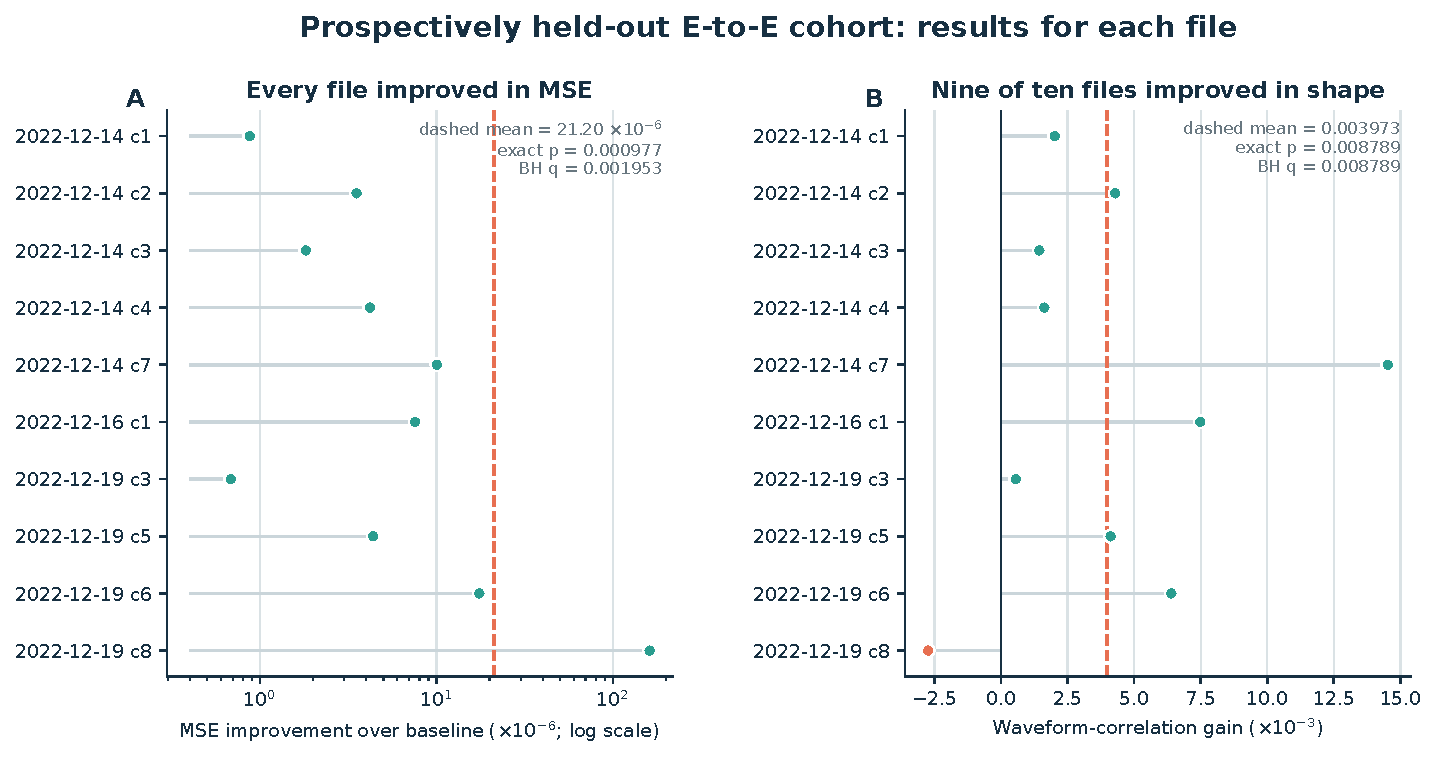
\includegraphics[width=0.97\textwidth]{figure3_primary_effects.pdf}
  \caption{\textbf{Main results in the new E-to-E data.}
  \textbf{A}, MSE improves in all ten files when neuron identity is added to
  the baseline. The log axis shows the full range. \textbf{B}, Waveform
  correlation improves in nine files. Dashed lines show the mean across
  files. Statistical tests treat files, not individual trials, as the units
  of evidence. File independence at the animal or slice level cannot be
  established from the public metadata.}
  \label{fig:effects}
\end{figure*}

\begin{table*}[t]
  \centering
  \caption{\textbf{Results of the prospectively held-out E-to-E test.} LOO is the
  smallest mean effect after leaving out one file.}
  \label{tab:confirmation}
  \resizebox{0.92\textwidth}{!}{\begin{tabular}{@{}lrrrrr@{}}
\toprule
Measure & Mean improvement & Files improved & Exact $p$ & Corrected $q$ & Smallest LOO \\
\midrule
MSE gain & 2.120e-05 & 10/10 & 0.000977 & 0.001953 & 5.619e-06 \\
Waveform $\Delta\rho$ & 0.00397 & 9/10 & 0.008789 & 0.008789 & 0.00280 \\
\midrule
MSE cost of using the wrong neuron & 4.567e-06 & 10/10 & 0.000977 & -- & -- \\
\bottomrule
\end{tabular}
}
\end{table*}

\subsection{Biological grouping is not identified in the public files}

The ten filenames identify recorded cells on three acquisition dates: five
files from 14 December 2022, one from 16 December, and four from 19 December.
The embedded field named \texttt{mouseID} contains labels such as
\texttt{cell3\_emx\_map}; it does not identify animals or slices. The public
files therefore support file-level comparisons across ten recorded cells but
do not establish ten independent biological preparations.

As a conservative sensitivity analysis, file effects were averaged within
the three dates before testing. The MSE and correlation effects remained
positive on all three dates. With only three date groups, however, the
smallest possible one-sided exact $p$ value is $0.125$. Acquisition date is
not claimed to be an animal or slice identifier; this calculation shows how
the inferential strength changes under a coarser plausible grouping. A
verified file-to-slice-to-animal map is required for biological-level
inference.

\subsection{The prediction required the correct neuron identities}

Improvement could arise because neuron-specific responses have a useful range
of sizes, even when assigned to the wrong neurons. To test this possibility,
neuron identities were shuffled within each imaging depth and laser power. The
shuffle preserved the response set, group sizes, powers, and recorded cell.
Across 999 fixed repetitions per file, the observed MSE and correlation
effects gave $z=29.47$ and $z=35.93$. Both were far above the familywise
99th-percentile threshold of $z=2.93$ (both familywise $p=0.001$;
Fig.~\ref{fig:identity}, Table~\ref{tab:identity}).

A second control replaced each stimulated neuron with matched unstimulated
neurons at the same depth and power. This replacement increased MSE in all
ten files (mean cost $4.57\times10^{-6}$, exact $p=0.0009766$). Together,
these controls show that power, depth, response size, and group size were not
enough. Improvement required assigning each response to the correct neuron.

\begin{figure*}[t]
  \centering
  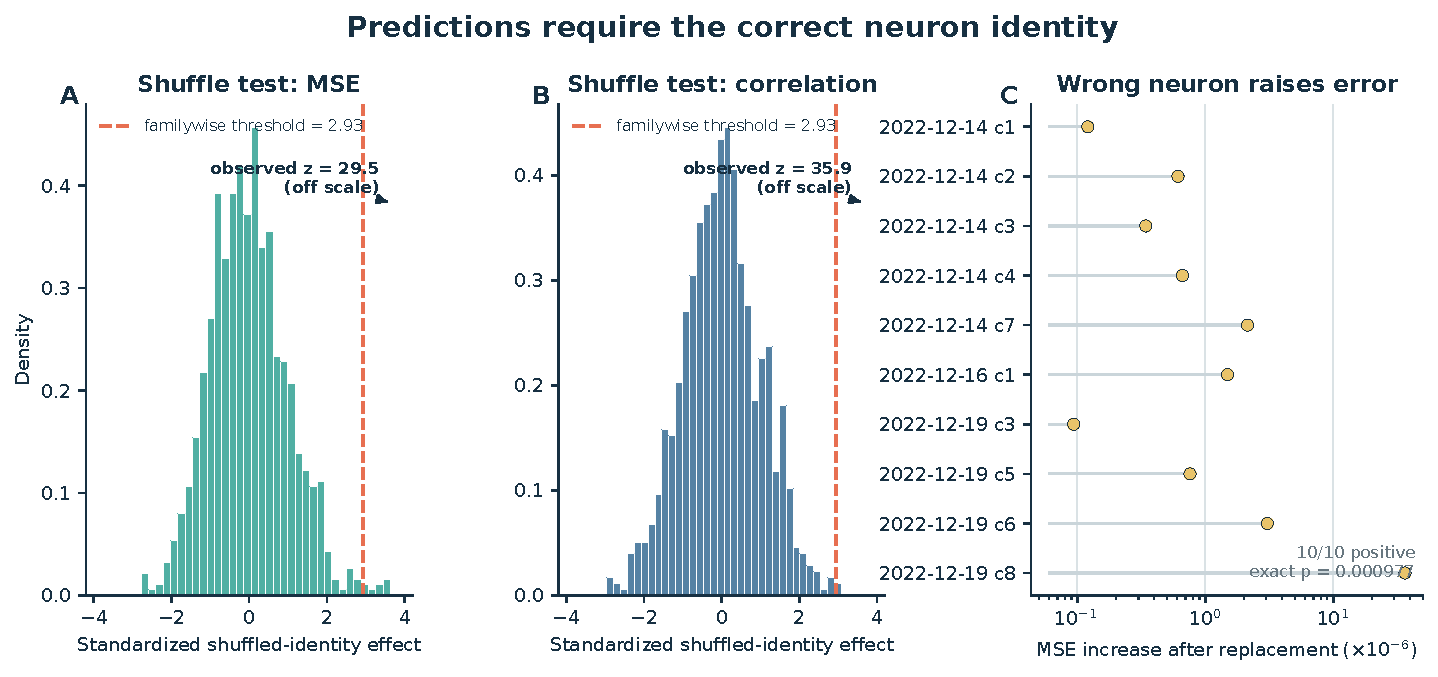
\includegraphics[width=\textwidth]{figure4_identity_ablation.pdf}
  \caption{\textbf{Controls for neuron identity.}
  \textbf{A--B}, Null effects from 999 identity shuffles that preserve depth
  and power. The observed statistics are far beyond the plotted nulls and
  the familywise threshold. \textbf{C}, Replacing a stimulated neuron with
  matched unstimulated neurons increases MSE in every file.}
  \label{fig:identity}
\end{figure*}

\begin{table}[t]
  \centering
  \caption{\textbf{Familywise tests of neuron identity.}}
  \label{tab:identity}
  \resizebox{\columnwidth}{!}{\begin{tabular}{@{}lrrr@{}}
\toprule
Measure & Observed $z$ & Familywise threshold & Familywise $p$ \\
\midrule
MSE gain & 29.47 & 2.93 & 0.001 \\
Waveform $\Delta\rho$ & 35.93 & 2.93 & 0.001 \\
\bottomrule
\end{tabular}
}
\end{table}

\subsection{Strength and latency explain the predictive improvement}

The full model allows every neuron to have a different waveform. A simpler
post-feedback model allowed only a neuron-specific scalar gain while forcing
all neurons at one power to share the same temporal shape. The gain was fit
by least-squares projection of each reliability-weighted single-neuron
response onto the shared waveform. This model used no group responses.

Source-specific gain improved demixed MSE over the power-only baseline in all
ten files (mean gain $2.051\times10^{-5}$, exact $p=0.000977$). This is 96.7\%
of the full model's mean MSE gain. Because a scalar does not change waveform
correlation, the gain-only model had the same correlation as the power-only
baseline. A second reduced model allowed the shared waveform to shift by up
to 2 ms for each neuron. Gain plus latency recovered a mean correlation gain
of $0.00190$ and nearly all MSE improvement ($2.119\times10^{-5}$).

Relative to gain plus latency, the full waveform changed mean MSE by only
$6.27\times10^{-9}$ ($p=0.495$) and correlation by $0.00207$ ($p=0.104$).
Thus the data clearly support source-specific response strength. They also
suggest temporal information, but do not show that unrestricted waveform
detail predicts groups better than the simpler gain-and-latency model
(Fig.~\ref{fig:reduced}, Table~\ref{tab:reduced}).

\begin{figure*}[t]
  \centering
  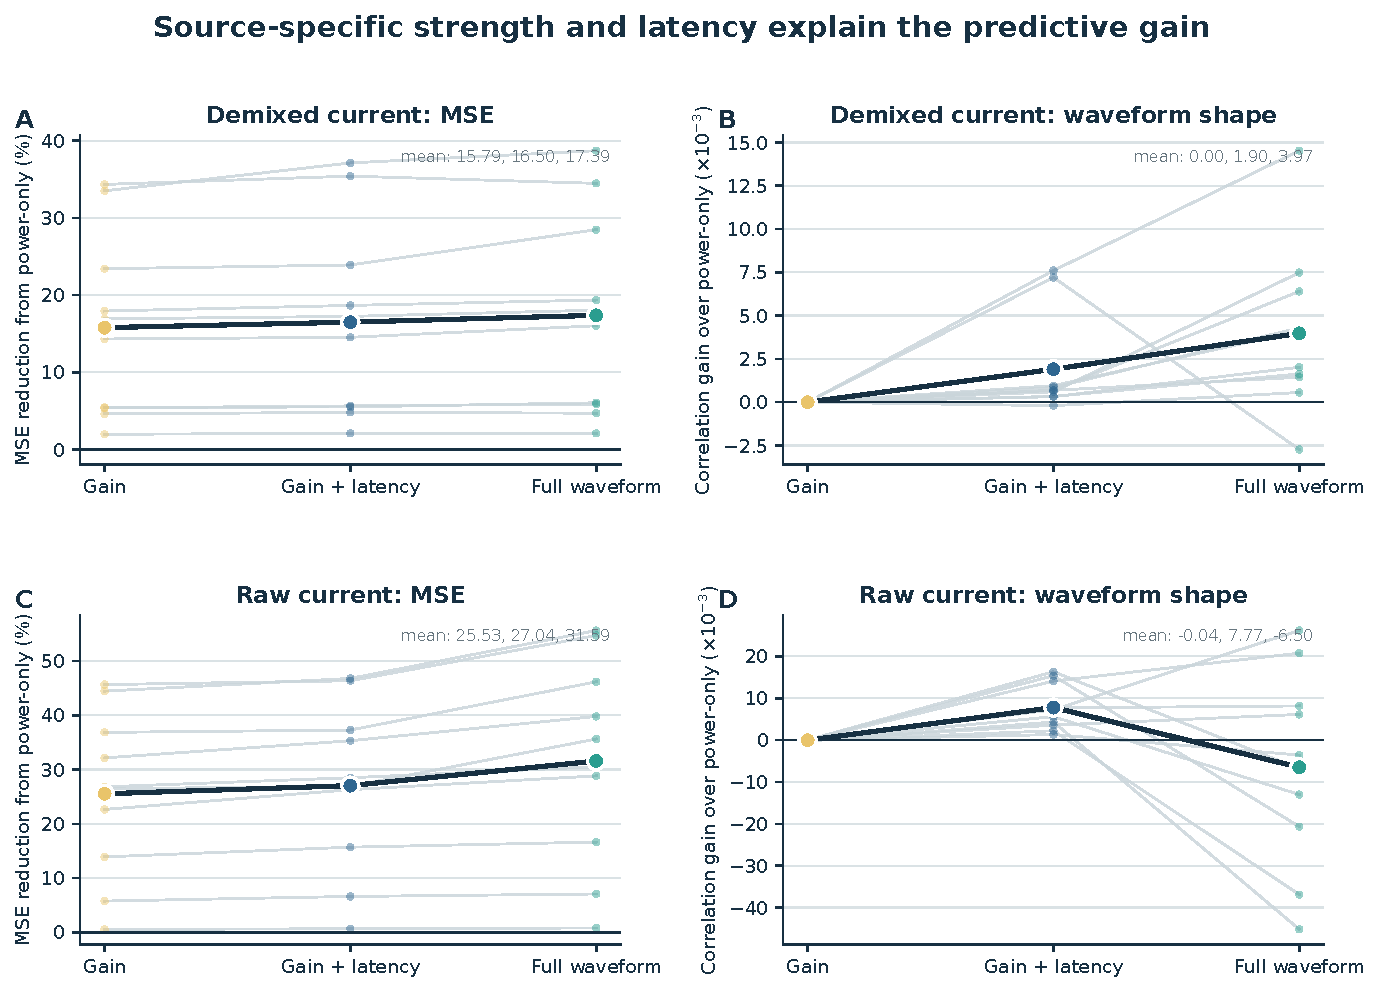
\includegraphics[width=0.98\textwidth]{figure6_reduced_models.pdf}
  \caption{\textbf{Which single-neuron information is needed?}
  Thin lines show files and large points show equal-file means. MSE panels
  report percentage reduction from the power-only baseline; correlation
  panels report the absolute gain. \textbf{A--B}, NWD-demixed current.
  \textbf{C--D}, Raw current. Source-specific gain explains most MSE
  improvement. Gain plus latency improves correlation in demixed and raw
  current; unrestricted waveform detail does not add a conclusive advantage.}
  \label{fig:reduced}
\end{figure*}

\begin{table*}[t]
  \centering
  \caption{\textbf{Post-feedback reduced-model comparison on demixed
  current.} Gains are relative to the power-only model. All reduced-model
  parameters were learned from single-neuron trials only.}
  \label{tab:reduced}
  \resizebox{0.88\textwidth}{!}{\begin{tabular}{@{}lrrrr@{}}
\toprule
Single-neuron model & Mean MSE & MSE gain & Mean $\rho$ & $\Delta\rho$ \\
\midrule
Power only & 8.204e-05 & -- & 0.4070 & -- \\
Source gain & 6.153e-05 & 2.051e-05 & 0.4070 & 0.00000 \\
Source gain $+$ latency & 6.085e-05 & 2.119e-05 & 0.4089 & 0.00190 \\
Full waveform & 6.084e-05 & 2.120e-05 & 0.4109 & 0.00397 \\
\bottomrule
\end{tabular}
}
\end{table*}

\subsection{Reliability changed with power and preparation}

The model did not assume that every neuron-specific difference was reliable.
Mean $\lambda$ was $0.479$ in the demixed E-to-E data, compared with $0.781$
in the SST development data. In E-to-E files, mean reliability rose from
$0.264$ at power 30 to $0.504$ at power 45 and $0.670$ at power 60
(Fig.~\ref{fig:reliability}). Two low-power estimates fell to zero, while one
high-signal file kept more than $0.84$ at every power. Predictions were
therefore closer to the shared response when neuron-specific differences did
not repeat, while repeatable differences were retained.

\begin{figure*}[t]
  \centering
  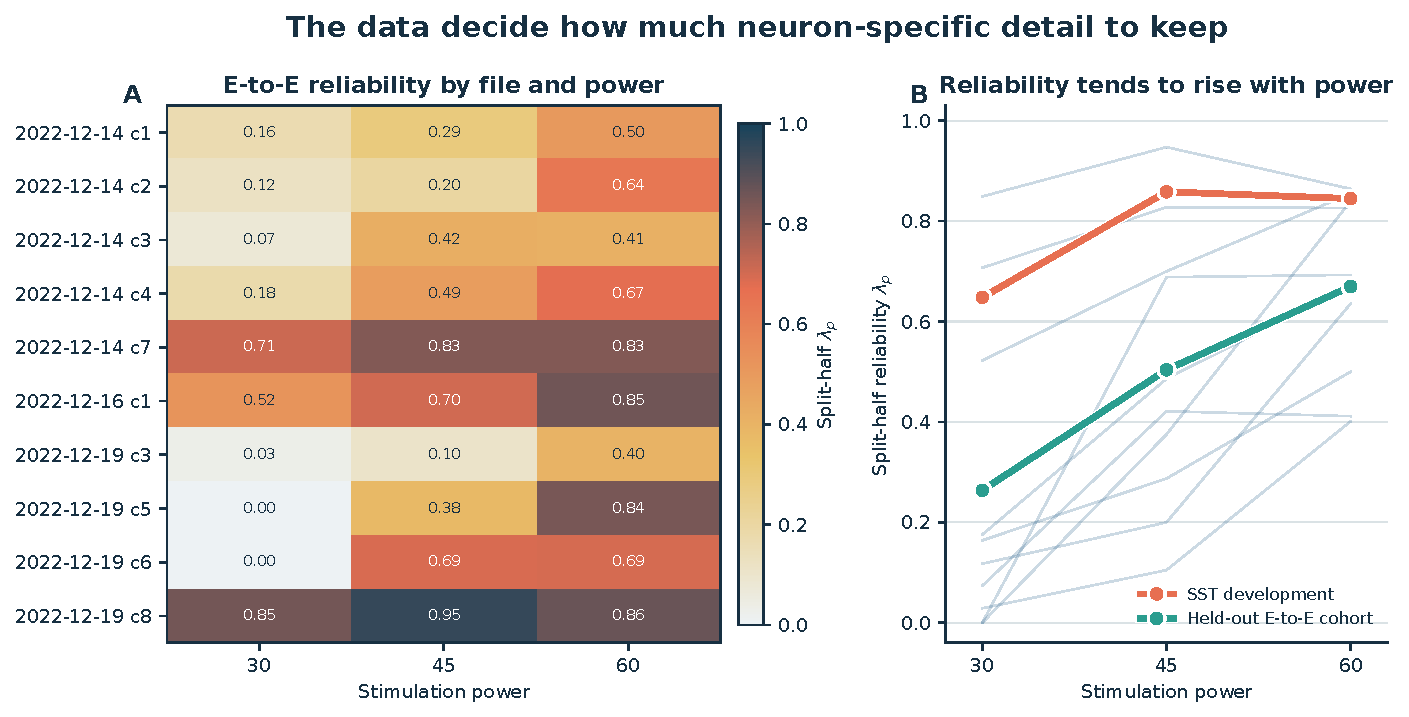
\includegraphics[width=0.96\textwidth]{figure5_reliability.pdf}
  \caption{\textbf{Reliability controls how much neuron-specific detail is
  kept.} \textbf{A}, E-to-E reliability values by file and laser power.
  \textbf{B}, Thin lines show individual E-to-E files; thick lines show the
  mean across files. Reliability rises with power in E-to-E data and is lower
  than in the SST development data.}
  \label{fig:reliability}
\end{figure*}

\subsection{The reduced model reveals a raw-current latency effect}

In the preregistered full-waveform comparison, two supporting measures,
integrated-current error and peak-current error,
improved in all ten E-to-E files (post-hoc three-outcome $q=0.00146$ for
each). Raw-current MSE also improved, but raw waveform correlation did not
($q=0.803$). The claim about waveform shape therefore depends on NWD
demixing.

Mean waveform correlation was $0.4109$ for the neuron-specific model and
$0.4070$ for the baseline. Mean MSE was $6.1\times10^{-5}$ for the
neuron-specific model, $8.2\times10^{-5}$ for the baseline, and
$1.03\times10^{-4}$ for zero. The file-level comparison with zero varied
across preparations (4/10 positive, exact $p=0.456$), as small currents make
zero competitive under squared error.

The reduced-model sensitivity sharpened this result. On raw current,
source-specific gain improved MSE in all ten files but did not improve mean
correlation. Gain plus latency improved both raw MSE and raw correlation in all
ten files (mean correlation gain $0.00777$, exact $p=0.000977$). The
unrestricted full waveform improved raw MSE further, but its mean correlation
remained below the power-only baseline. Thus source-specific strength and
latency both transfer to the direct physical recordings; arbitrary residual
waveform detail does not.

\section{Discussion}

This reanalysis identifies a narrow, repeatable predictive effect. Responses
learned from single-neuron stimulation improve predictions of held-out group
current, and the improvement requires the correct neuron identities. The
reduced-model comparison shows what carries most of that effect: some neurons
produce reliably stronger postsynaptic responses than others at the same
laser power. Those source-specific strengths remain useful when the neurons
are stimulated in groups.

The temporal result is narrower than a general waveform claim. A
source-specific latency shift improves correlation in both demixed and raw
current, while the unrestricted waveform does not conclusively outperform
gain plus latency. NWD does not receive neuron identity or fit the
single-neuron templates used here, so the analysis is not a direct projection
of group responses onto those templates. NWD is nevertheless trained on
simulated PSC-like waveforms and favors clean evoked-current structure
\citep{triplett2025rapid}. Conclusions about residual waveform detail, beyond
gain and latency, should therefore remain conditional on preprocessing.

The result differs from the leave-one-hologram-out prediction in the source
study. CAVIaR learned from responses to other group holograms; the present
models learn only from single-neuron trials. The new contribution is thus not
that currents can be added or that an unseen hologram can be predicted. It is
that source-specific response strength and latency transfer from individual
stimulation to withheld group stimulation without fitting any group response.

The prospective separation between SST development and E-to-E testing
protects against adapting the rule to the E-to-E responses. It does not by
itself establish biological independence. The ten files are ten recorded
postsynaptic cells, but their animal and slice membership is absent from the
public metadata. The three-date sensitivity preserves the direction of the
effect but cannot provide a small exact $p$ value. Biological-level inference
requires the missing hierarchy.

\subsection{Next steps and opportunities}

The immediate next step is to obtain the anonymized mapping from files to
slices and animals, then repeat the sign-flip tests and leave-one-out analysis
at the highest independent biological level. This requires no new response
analysis and directly determines the strength of the population-level claim.

A new preregistered comparison should then test the model hierarchy found
here: power only, source gain, source gain plus latency, and unrestricted
waveform. Applying that fixed hierarchy to another source-cell class would
show whether latency or residual temporal detail generalizes beyond this
post-feedback analysis.

The present models learn a separate response for every neuron and exact laser
power. Holding out one neuron--power pair and predicting it from the same
neuron at other powers would test whether source strength follows a rule
across stimulation intensity rather than acting as an exact-power lookup.

A second experiment should be designed to distinguish addition from competing
models. Repeated stimulation of selected pairs and progressively larger groups
could compare the additive rule with saturation, pairwise interaction, and
gain-control models on combinations withheld from fitting. The pattern of
errors would then reveal not only whether additive predictions remain accurate,
but also where and how they give way to another response rule.

Temporal prediction should also be tested under recording conditions chosen
for direct analysis of raw current. Longer intervals between stimuli, repeated
presentations of the same groups, and source-blind filtering would reduce
overlapping events and electrical noise without using neuron identity. These
experiments would test whether residual waveform detail beyond strength and
latency transfers to physical recordings.

Predictive models can also distinguish biological explanations.
Direct measurements of presynaptic spiking could separate variable optical
activation from variable synaptic transmission. Postsynaptic holding-potential
changes and receptor-specific perturbations could test whether departures from
addition arise from driving force, receptor recruitment, or recurrent
interactions. Experiments should be selected so that candidate models make
different predictions before the responses are observed.

Together, the results support a compact predictive rule: source-specific
response strength and latency learned from individual stimulation improve
held-out group-current prediction. Unrestricted temporal detail remains an
open test.

\section{Methods}

\subsection{Public recordings and locked datasets}

All recordings came from the CC BY 4.0 Figshare dataset
``Neural circuit mapping using two-photon holographic optogenetics,''
version 1 \citep{gajowa2025dataset}, associated with
\citet{triplett2025rapid}. The upstream analysis-code reference was frozen at
\texttt{marcustriplett/circuitmap} commit
\texttt{75934895f8ef02b8045ab1a8eee592a062c2489e}.
The development manifest contained all nine SST-to-E files. The prospectively
held-out manifest contained all ten E-to-E files. URLs, file sizes, and checksums
were recorded before analysis. Fourteen PV-to-E files remained unopened
because the planned SST waveform criterion was not met.

Each MATLAB v7.3/HDF5 file contained a trial-by-neuron
\texttt{stimulus\_matrix}, trial-by-time raw and demixed current arrays
(\texttt{pscs}, \texttt{pscs\_demixed}), and neuron coordinates
(\texttt{targets}). CAVIaR weight fields were checked only to validate the
file structure. They were not used to
predict, filter, label, or select trials.

\subsection{Learning trials, test trials, and response window}

A single-neuron trial had exactly one positive stimulus entry. A group trial
had more than one, and blank trials were excluded. Single-neuron trials were
used only to learn responses and reliability. Group trials were used only
for evaluation. Each trace had 900 samples at 20 kHz, with stimulation at
sample 100. For each trial, the mean of samples 0--99 was subtracted and
samples 120--899, or 1--40 ms after stimulation, were analyzed. The first
post-stimulus millisecond was excluded. NWD-demixed current was the main
outcome; raw current was a supporting outcome.

A trace containing only nonfinite values was allowed only for a blank trial,
which was then excluded. Any partly nonfinite trace or nonfinite stimulated
trial failed validation. Laser powers were not grouped into bins. Learning a
response for one neuron at one power required at least three single-neuron
trials. A group trial was eligible only when every stimulated neuron met this
requirement at its exact delivered power.

\subsection{Neuron-specific and baseline models}

Let $\bar{K}_{s,p}(t)$ be the mean response across single-neuron trials for
neuron $s$ at exact power $p$. The baseline response was the mean across
neurons, giving every neuron equal weight rather than weighting by its number
of trials:
\begin{equation}
g_p(t)=\frac{1}{|S_p|}\sum_{s\in S_p}\bar{K}_{s,p}(t),
\end{equation}
The neuron-specific difference was
$d_{s,p}(t)=\bar{K}_{s,p}(t)-g_p(t)$.

To estimate reliability, trials for each $(s,p)$ pair were assigned in stored
order to alternating halves. Let $A_{s,p}(t)$ and $B_{s,p}(t)$ be the two
half means. Each half was centered independently across neurons:
$A'_{s,p}=A_{s,p}-|S_p|^{-1}\sum_s A_{s,p}$ and analogously for $B'$.
For each file, outcome, and power,
\begin{equation}
\lambda_p =
\left[
\frac{2\sum_{s,t} A'_{s,p}(t)B'_{s,p}(t)}
{\sum_{s,t}A'_{s,p}(t)^2+\sum_{s,t}B'_{s,p}(t)^2}
\right]_{0}^{1}.
\end{equation}
The brackets limit the value to $[0,1]$. After determining $\lambda_p$, the
final response followed Eq.~\ref{eq:response} and used the mean of all
single-neuron trials.

For an eligible group $E$, the baseline added $g_{p_s}(t)$ for the stimulated
neurons. The neuron-specific model used Eq.~\ref{eq:sum}. A zero waveform was
included as a supporting baseline. Group responses were not used to fit an
intercept, coefficient, gain, latency shift, saturation term, time window,
rank, or neuron filter.

\subsection{Reduced models added after external feedback}

The gain-only model was constructed from the frozen reliability-weighted
response $r_{s,p}$ and the shared waveform $g_p$. For every source and power,
the least-squares scalar was
\begin{equation}
\alpha_{s,p}=\left[
\frac{\langle r_{s,p},g_p\rangle}
{\langle g_p,g_p\rangle}\right]_{0}^{\infty},
\end{equation}
and the reduced response was $\alpha_{s,p}g_p(t)$. Negative projections were
set to zero; if $g_p$ had zero energy, $\alpha_{s,p}$ was set to one. The
gain-plus-latency model shifted $g_p$ by
each integer lag from $-40$ to $40$ samples ($\pm2$ ms), refit $\alpha$ for
each lag, and retained the pair with the smallest single-neuron waveform
error. No group response selected a gain, lag, or model.

These reduced models and their comparisons were specified after external
feedback and are reported as sensitivity analyses, not as part of the locked
E-to-E gate. Exact sign-flip tests used the same equal-file aggregation as
the original analysis.

\subsection{Biological-unit audit and date sensitivity}

The filename supplied the acquisition date and recorded-cell label. The
MATLAB \texttt{ExpStruct.mouseID} field was read directly from every E-to-E
file, but its values repeated cell labels rather than animal identifiers. No
slice identifier was found. To show the consequence of possible clustering,
file effects were averaged within acquisition date and the exact sign-flip
test was repeated across the three dates. Date was used only as a conservative
session proxy and was not interpreted as a verified animal or slice.

\subsection{Measurements and statistical tests}

Four measures were calculated for each eligible trial: response-window MSE,
Pearson waveform correlation, absolute error in integrated current, and
absolute error in peak current. Correlation was set to zero when either
waveform was constant.
Integrated current was the response-window sum multiplied by 0.05 ms. Peak
current was the signed sample with the largest absolute value.

The two main effects were baseline MSE minus neuron-specific MSE and
neuron-specific correlation minus baseline correlation. Trial-level effects
were first averaged within each file. Across files, exact one-sided sign-flip
tests considered all $2^n$ sign assignments \citep{fisher1935design}. The two
main $p$ values were corrected by Benjamini--Hochberg
\citep{benjamini1995controlling}. Both equal-file means had to be positive
with $q<0.05$. Each effect also had to remain positive after leaving out any
one file.

\subsection{Identity shuffling and matched-neuron replacement}

For each of 999 fixed null repetitions per file, neuron identities were
shuffled separately within imaging depth and exact power. The same shuffle
was applied to all group trials in one repetition. This kept power, depth,
group size, recorded cell, and the set of learned responses unchanged. Null
effects gave every file equal weight. Because MSE and correlation use
different units, each was standardized using its own null mean and standard
deviation. The larger standardized value from the two measures formed a
familywise null. Both observed $z$ scores had to exceed its 99th percentile.

The replacement test asked whether each correct identity was necessary. Each
stimulated neuron was replaced in turn by every eligible unstimulated neuron
at the same depth and exact power. Replacement MSE minus the original MSE was
averaged across replacements, stimulated neurons, trials, and then files. A
positive exact one-sided sign-flip test across files was required.

\subsection{Reproducibility}

The public repository contains frozen protocols and lock records, raw-data
manifests, analysis and download code, unit tests, compact derived tables,
figure builders, and this manuscript. All figures are generated from the
included CSV and JSON outputs. Reproducing the complete analysis requires
downloading about 2.01 GiB of SST recordings and 7.64 GiB of E-to-E
recordings. The repository does not redistribute the raw recordings.

\section*{Data and code availability}

Source data are available from Figshare at
\url{https://doi.org/10.6084/m9.figshare.25641435.v1}. The reproducible
manuscript repository is
\url{https://github.com/asim-v/holographic-source-grammar}. Code is released
under MIT; original manuscript materials and derived tables are CC BY 4.0.

\section*{Ethics statement}

This study is a secondary analysis of public data and introduced no new
animal experiments. Animal procedures and approvals are described in the
source publication \citep{triplett2025rapid}.

\section*{Acknowledgments}

The author thanks Marta Gajowa, Marcus Triplett, and colleagues for releasing
the recordings and software that made this independent reanalysis possible.

\section*{Author contributions}

J.E.B.S. conceived the reanalysis, designed the protocols, implemented and
validated the software, analyzed the data, prepared the visualizations, and
wrote the manuscript.

\section*{Funding}

No specific funding was received for this reanalysis.

\section*{Competing interests}

The author declares no competing interests.

\balance
\bibliographystyle{plainnat}
\bibliography{references}

\end{document}
